\section{Selecting the Sample Size}

For our C.I. we have $\that\pm Z_{\alpha/2}\sigma_{\that}$
    \begin{itemize}
        \item $\sigma_{\that}$ is the standards error
        \item $E = Z_{\alpha/2}\sigma_{\that}$ is the error bounds of our C.I.
    \end{itemize}
    In real world, we choose our confidence level $1-\alpha$ and/or the error $E$ ahead of time. This leads to the problem of choosing an appropriate sample size $n$.
    
    \example For $\bar{X}, \dots$ distributions is $\normalDist*$.
    $$\sigma_{\Xbar} = \sqrt{\sigma^2/n} \qquad \text{and} \qquad E = Z_{\alpha/2} \sqrt{\sigma^2/n}$$
    $$\longleftrightarrow\quad n = \frac{Z_{\alpha/2}\sigma^2}{E^2}$$
    For desired $E$, we need to choose
    $$n \geq \left\lceil \frac{Z_{\alpha/2}\sigma^2}{E^2}\right\rceil$$
    Another issue: We don't really know ${\sigma_{\that}}^2$ and maybe not even $Z_{\alpha/2}$.

    \begin{enumerate}[label=\textcircled{\raisebox{-1pt}{\arabic*}}]
        \item For $Z_{\alpha/2}$, we have seen that the empirical rule $2\sigma$ usually works for large $n$.
        \begin{center}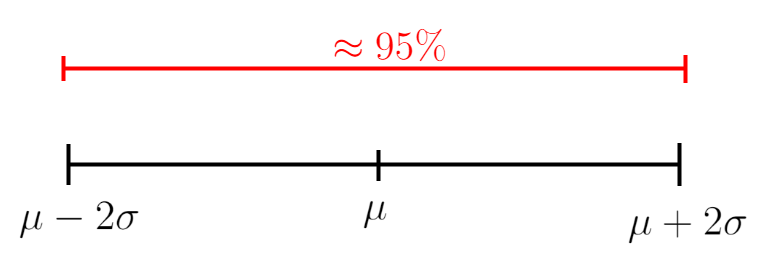
\includegraphics[width=4in]{2 sigma.png}\end{center}

        \item For $\sigma_{\that}$, either
        \begin{enumerate}[label=\textbf{{\alph*}.)}]
            \item Use old data or a \say{pilot} sample $S^2$
            \item Use $\over{4}$ the spread of the data set, i.e.,
            $$\sigma_{\that} \approx \over{4} \big( \operatorname{max}(Y_i)-\operatorname{min}(Y_i)\big) $$
        \end{enumerate}
    \end{enumerate}
    However, for proportions we can do even better.

    \example Proportions. For 
    $\phat = \dfrac{\displaystyle \sum Y_i}{n} \hspace{0.25in} \text{(relative frequency)}$,  
    $\;\phat$ distributed $N\pars{p, \dfrac{pq}{n}}$
    $$E = Z_{\alpha/2} \sqrt{\frac{pq}{n}} \hspace{.5in} \longleftrightarrow \hspace{0.5in} n \geq \left\lceil \frac{Z_{\alpha/2}^2p(1-p)}{E^2}\right\rceil $$
    Again, since $p(1-p) \leq \dfrac{1}{4}$ on $[0,\,1]$, we choose $n \geq \dfrac{Z_{\alpha/2}^2}{4E}$

    \newpage \noindent \example* Public opinion polls ($\pm 3\%$)

    \nnl For a 95\% Confidence interval,
    $$Z_{\alpha/2} = 1.960 \qquad \text{and} \qquad n \geq \ceiling{\frac{1.96^2}{4(0.03)^2}} = 1068$$

    \nnl For a 99\% Confidence interval,
    $$Z_{\alpha/2} = 2.576 \qquad \text{and} \qquad n \geq \ceiling{\frac{2.576^2}{4(0.03)^2}} = 1844$$